\documentclass[border=12pt]{standalone}
\usepackage{tikz}
\usetikzlibrary{arrows.meta, positioning, calc, fit, backgrounds}
\usepackage{amsmath, amssymb}

\begin{document}
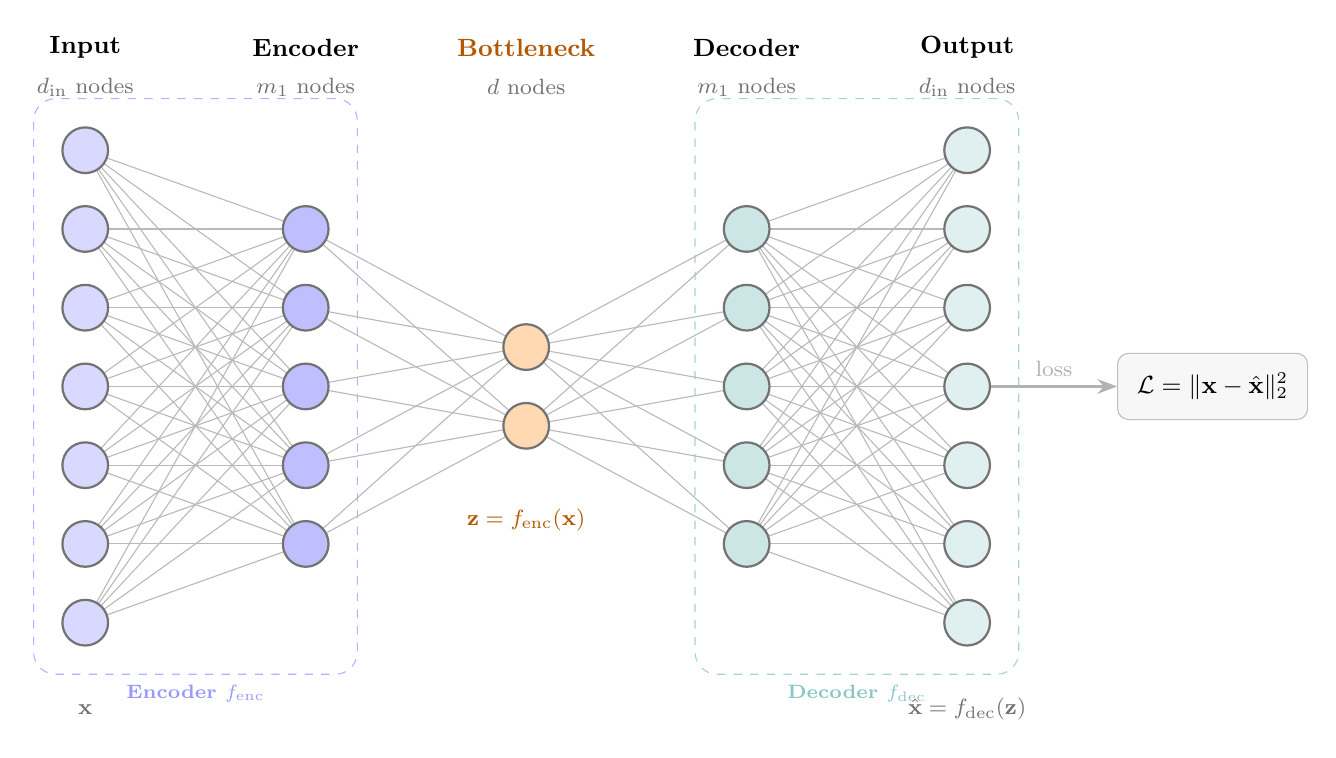
\begin{tikzpicture}[
    neuron/.style = {circle, draw=black!55, thick, minimum size=0.58cm, inner sep=0pt},
    inp/.style    = {neuron, fill=blue!15},
    enc/.style    = {neuron, fill=blue!25},
    bot/.style    = {neuron, fill=orange!30},
    dec/.style    = {neuron, fill=teal!20},
    outp/.style   = {neuron, fill=teal!12},
    conn/.style   = {draw=gray!55, line width=0.4pt},
    arr/.style    = {-{Stealth[length=2.5mm]}, thick},
]

%% ---- Layer positions (x-coords) ----
\def\xI{0}       % input
\def\xE{2.8}     % encoder hidden
\def\xB{5.6}     % bottleneck
\def\xD{8.4}     % decoder hidden
\def\xO{11.2}    % output (reconstruction)

%% ---- Node counts ----
% Input: 7, Encoder: 5, Bottleneck: 2, Decoder: 5, Output: 7

%% ---- Edges first (behind nodes) ----
% Input -> Encoder
\foreach \i in {1,...,7}{
    \foreach \e in {1,...,5}{
        \draw[conn] (\xI, {4-\i}) -- (\xE, {3-\e});
    }
}
% Encoder -> Bottleneck
\foreach \e in {1,...,5}{
    \foreach \b in {1,...,2}{
        \draw[conn] (\xE, {3-\e}) -- (\xB, {1.5-\b});
    }
}
% Bottleneck -> Decoder
\foreach \b in {1,...,2}{
    \foreach \d in {1,...,5}{
        \draw[conn] (\xB, {1.5-\b}) -- (\xD, {3-\d});
    }
}
% Decoder -> Output
\foreach \d in {1,...,5}{
    \foreach \o in {1,...,7}{
        \draw[conn] (\xD, {3-\d}) -- (\xO, {4-\o});
    }
}

%% ---- Nodes ----
\foreach \i in {1,...,7}{ \node[inp]  (I\i) at (\xI, {4-\i}) {}; }
\foreach \e in {1,...,5}{ \node[enc]  (E\e) at (\xE, {3-\e}) {}; }
\foreach \b in {1,...,2}{ \node[bot]  (B\b) at (\xB, {1.5-\b}) {}; }
\foreach \d in {1,...,5}{ \node[dec]  (D\d) at (\xD, {3-\d}) {}; }
\foreach \o in {1,...,7}{ \node[outp] (O\o) at (\xO, {4-\o}) {}; }

%% ---- Layer labels (top) ----
\node[font=\small\bfseries]         at (\xI, 4.3) {Input};
\node[font=\footnotesize, black!55] at (\xI, 3.8) {$d_{\mathrm{in}}$ nodes};

\node[font=\small\bfseries]         at (\xE, 4.3) {Encoder};
\node[font=\footnotesize, black!55] at (\xE, 3.8) {$m_1$ nodes};

\node[font=\small\bfseries, orange!70!black] at (\xB, 4.3) {Bottleneck};
\node[font=\footnotesize, black!55] at (\xB, 3.8) {$d$ nodes};

\node[font=\small\bfseries]         at (\xD, 4.3) {Decoder};
\node[font=\footnotesize, black!55] at (\xD, 3.8) {$m_1$ nodes};

\node[font=\small\bfseries]         at (\xO, 4.3) {Output};
\node[font=\footnotesize, black!55] at (\xO, 3.8) {$d_{\mathrm{in}}$ nodes};

%% ---- Bottom labels ----
\node[font=\footnotesize, black!55, align=center] at (\xI, -4.1) {$\mathbf{x}$};
\node[font=\footnotesize, orange!70!black, align=center] at (\xB, -1.7) {$\mathbf{z} = f_{\mathrm{enc}}(\mathbf{x})$};
\node[font=\footnotesize, black!55, align=center] at (\xO, -4.1) {$\hat{\mathbf{x}} = f_{\mathrm{dec}}(\mathbf{z})$};

%% ---- Encoder / Decoder grouping braces ----
\begin{scope}[on background layer]
    \node[draw=blue!30, dashed, rounded corners=8pt, inner sep=10pt,
          fit=(I1)(I7)(E1)(E5),
          label={[font=\scriptsize\bfseries, blue!40]below:Encoder $f_{\mathrm{enc}}$}] {};
    \node[draw=teal!35, dashed, rounded corners=8pt, inner sep=10pt,
          fit=(D1)(D5)(O1)(O7),
          label={[font=\scriptsize\bfseries, teal!45]below:Decoder $f_{\mathrm{dec}}$}] {};
\end{scope}

%% ---- Loss annotation ----
\node[draw=gray!50, rounded corners=4pt, fill=gray!6, font=\small,
      right=1.6cm of O4, align=center, inner sep=7pt] (loss)
    {$\mathcal{L} = \|\mathbf{x} - \hat{\mathbf{x}}\|_{2}^{2}$};

\draw[arr, gray!60] (O4.east) -- (loss.west)
    node[midway, above, font=\footnotesize] {loss};

\end{tikzpicture}
\end{document}
